\documentclass[DIV=21,a3,landscape,9pt]{scrartcl}\usepackage[]{graphicx}\usepackage[]{xcolor}
% maxwidth is the original width if it is less than linewidth
% otherwise use linewidth (to make sure the graphics do not exceed the margin)
\makeatletter
\def\maxwidth{ %
  \ifdim\Gin@nat@width>\linewidth
    \linewidth
  \else
    \Gin@nat@width
  \fi
}
\makeatother

\definecolor{fgcolor}{rgb}{0.345, 0.345, 0.345}
\newcommand{\hlnum}[1]{\textcolor[rgb]{0.686,0.059,0.569}{#1}}%
\newcommand{\hlstr}[1]{\textcolor[rgb]{0.192,0.494,0.8}{#1}}%
\newcommand{\hlcom}[1]{\textcolor[rgb]{0.678,0.584,0.686}{\textit{#1}}}%
\newcommand{\hlopt}[1]{\textcolor[rgb]{0,0,0}{#1}}%
\newcommand{\hlstd}[1]{\textcolor[rgb]{0.345,0.345,0.345}{#1}}%
\newcommand{\hlkwa}[1]{\textcolor[rgb]{0.161,0.373,0.58}{\textbf{#1}}}%
\newcommand{\hlkwb}[1]{\textcolor[rgb]{0.69,0.353,0.396}{#1}}%
\newcommand{\hlkwc}[1]{\textcolor[rgb]{0.333,0.667,0.333}{#1}}%
\newcommand{\hlkwd}[1]{\textcolor[rgb]{0.737,0.353,0.396}{\textbf{#1}}}%
\let\hlipl\hlkwb

\usepackage{framed}
\makeatletter
\newenvironment{kframe}{%
 \def\at@end@of@kframe{}%
 \ifinner\ifhmode%
  \def\at@end@of@kframe{\end{minipage}}%
  \begin{minipage}{\columnwidth}%
 \fi\fi%
 \def\FrameCommand##1{\hskip\@totalleftmargin \hskip-\fboxsep
 \colorbox{shadecolor}{##1}\hskip-\fboxsep
     % There is no \\@totalrightmargin, so:
     \hskip-\linewidth \hskip-\@totalleftmargin \hskip\columnwidth}%
 \MakeFramed {\advance\hsize-\width
   \@totalleftmargin\z@ \linewidth\hsize
   \@setminipage}}%
 {\par\unskip\endMakeFramed%
 \at@end@of@kframe}
\makeatother

\definecolor{shadecolor}{rgb}{.97, .97, .97}
\definecolor{messagecolor}{rgb}{0, 0, 0}
\definecolor{warningcolor}{rgb}{1, 0, 1}
\definecolor{errorcolor}{rgb}{1, 0, 0}
\newenvironment{knitrout}{}{} % an empty environment to be redefined in TeX

\usepackage{alltt}
%\usepackage{wasysym}
%\usepackage{amsmath,amssymb,amsthm}
%\usepackage{unicode-math}

% We set the Lucida OTF fonts as default
\usepackage{fontspec}
%\setmainfont{Lucida Bright OT}
\setmainfont{Lucida Sans OT}
\setsansfont{Lucida Sans OT}
\setmonofont{Lucida Console DK}[Scale=MatchLowercase]

%\newfontfamily\webglyphsfont{WebHostingHub-Glyphs}[Scale=0.7]
%\newcommand\webglyphs[1]{{\webglyphsfont\symbol{#1}}}
%\newcommand\Discussion{\colorbox{white}{\textcolor{black}{\webglyphs{"F134}}}\xspace}
%\newcommand\DiscussionI{\colorbox{black}{\textcolor{white}{\webglyphs{"F134}}}\xspace}
%\newcommand\DExamples{\colorbox{black}{\textcolor{white}{\webglyphs{"F134} examples?}}}
%\newcommand\Reading{\colorbox{black}{\textcolor{white}{\webglyphs{"F0C1}}}\xspace}
%\newcommand\ReadingI{\colorbox{white}{\textcolor{black}{\webglyphs{"F0C1}}}\xspace}
%\newcommand\Video{\colorbox{white}{\textcolor{black}{\webglyphs{"F03D}}}\xspace}
%\newcommand\Attention{\colorbox{black}{\textcolor{orange}{\webglyphs{"F05A}}}\xspace}
%\newcommand\HomeWork{\colorbox{white}{\textcolor{black}{\webglyphs{"F5ED}}}\xspace}
%\newcommand\HomeWorkI{\colorbox{black}{\textcolor{white}{\webglyphs{"F5ED}}}\xspace}
%\newcommand\Advanced{\colorbox{black}{\textcolor{white}{\webglyphs{"F235}}}\xspace}
%
%\newfontfamily\lineabasicfont{linea-basic-10}
%\newcommand\basicicons[1]{{\lineabasicfont\symbol{#1}}}
%\newcommand\timeforwards{\basicicons{"0079}}
%\newcommand\timebackwards{\basicicons{"0064}}
%
%\newfontfamily\lineaweatherfont{linea-weather-10}
%\newcommand\weathericons[1]{{\lineaweatherfont\symbol{#1}}}
%\newcommand\meteosun{\weathericons{"E038}}
%\newcommand\meteosuncloud{\weathericons{"E042}}
%\newcommand\meteorain{\weathericons{"E033}}
%\newcommand\meteowind{\weathericons{"E054}}
%
%\newfontfamily\uleaffont{Mini Pics Uprooted Leaf}
%\newcommand\uleafmpics[1]{{\uleaffont\symbol{#1}}}
%\newcommand\lowplants{\uleafmpics{"00CE}}
%\newcommand\mediumplant{\uleafmpics{"006A}}
%\newcommand\bush{\uleafmpics{"0039}}
%\newcommand\smallplant{\uleafmpics{"0030}}
%\newcommand\seedling{\uleafmpics{"002F}}
%\newcommand\floweringplant{\uleafmpics{"00CA}}
%
%\newfontfamily\utwigfont{Mini Pics Uprooted Twig}
%\newcommand\utwigmpics[1]{{\utwigfont\symbol{#1}}}
%\newcommand\grassplant{\utwigmpics{"0033}}
%
%\newfontfamily\uinsectfont{Insect Icons}
%\newcommand\uinsect[1]{{\uinsectfont\symbol{#1}}}
%\newcommand\bug{\uinsect{"006F}}

\usepackage{polyglossia}
\setdefaultlanguage[variant = british, ordinalmonthday = false]{english}

%\usepackage[style=authoryear-comp,firstinits,sortcites,maxcitenames=2,%
%    mincitenames=1,maxbibnames=10,minbibnames=10,uniquename=mininit,%
%    uniquelist=minyear,sortfirstinits=true]{biblatex}
%\addbibresource{../references/ecophys.bib}
%\renewcommand{\bibfont}{\small}

\usepackage{abbrev}
\DeclareGraphicsExtensions{.png,.jpg,.jpeg,.pdf}



\usepackage{multicol}
\setlength{\columnseprule}{1pt}
\usepackage{booktabs}

\usepackage[olditem]{paralist}%,oldenum

%\setlength{\parindent}{2em}
\pagestyle{myheadings}
\IfFileExists{upquote.sty}{\usepackage{upquote}}{}
\begin{document}

\title{\huge Plot insets and data labels with \textcolor{purple}{ggpp}\ :\,:\ CHEAT SHEET\hfill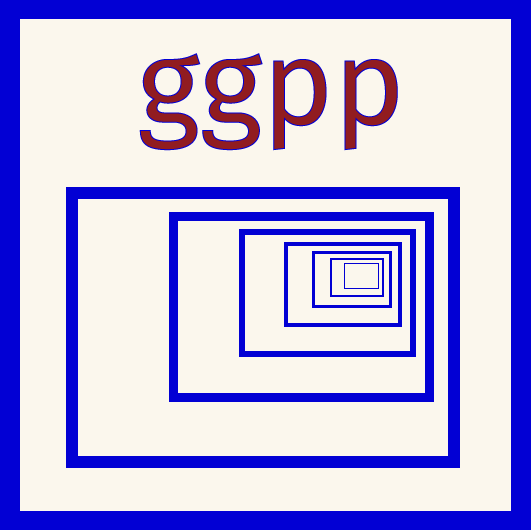
\includegraphics[width=3cm]{logo-ggpp.png}}
%\subtitle{Enhancements to the grammar of layered graphics}
%\author{Pedro J. Aphalo}
%\institute{University of Helsinki}
%\email{https://www.r4photobiology.info/}
%\conference{CHEAT SHEET.}
\date{\null}



\maketitle\vspace{-20mm}

\begin{multicols}{3}

\section*{Basics}

\textbf{ggpp} extends \textbf{ggplot2} and the \textbf{grammar of graphics} that it is based on. Plot construction remains unchanged but new \textbf{geometries}, \textbf{scales} and \textbf{positions} support the use of the same grammar as for observations for \emph{data labels} and \emph{annotations}. In the case of data labels, which are linked to observations, their, usually displaced, positions are meaningful in data units. Textual annotations and insets are, in contrast, linked to a plot as a whole, and their location within the plotting area decided on graphic design basis. True annotations and insets can be easily separated from the plot, while, data labels, cannot.



\section*{Plots, tables and grobs as labels}

A different plot, a table or an illustration set within the plotting area of a larger plot is called an \textsl{inset} when they are annotations, but if small, they can also function as data labels.

\textbf{geom\_plot()}, \textbf{geom\_table()}, and \textbf{geom\_grob()} differ from ggplot's \textbf{geom\_text()} mainly in that instead working by mapping a \texttt{character} vector to the \texttt{label} aesthetic, they require a list of \texttt{gg} objects, a list of \texttt{data.frame} objects or a list of \texttt{grob} objects to be mapped to \texttt{label}. While all geoms return trees or lists of \texttt{grob}s (or graphical objects) as defined in package 'grid', \textbf{geom\_grob()} accepts a list of \texttt{grob}s or grob trees mapped to the \texttt{label} aesthetic and collects them into a plot layer. (\texttt{grob}s can be built in advance using drawing functions or constructed by converting raster or vector graphics objects from other formats into \texttt{grob}s.)

As in \textbf{geom\_text()} \texttt{hjust} and \texttt{vjust} control the justification of each inset in whole. Rotation with \texttt{angle} is supported. Size can be adjusted in proportion to the plotting area with aesthetics \texttt{vp.width} and \texttt{vp.height}. Aesthetic \texttt{size} is not supported. \textbf{geom\_table()} accepts table themes (\textbf{ttheme}s), of which several are provided. \textbf{stat\_fmt\_tb()} makes it possible to select part of a data frame and/or replace headings when adding it as an inset with \textbf{geom\_table()}.\vspace{1ex}

\noindent
\textbf{ttheme\_gtdefault()}\\
\textbf{ttheme\_gtminimal()}\\
\textbf{ttheme\_gtbw()}\\
\textbf{ttheme\_gtplain()}\\
\textbf{ttheme\_gtdark()}\\
\textbf{ttheme\_gtlight()}\\
\textbf{ttheme\_gtsimple()}\\
\textbf{ttheme\_gtstripes()}

\section*{Annotations}

True annotations can be added using data coordinates or native plot coordinates (NPC) depending on the situation. NPC coordinates are specially useful when adding annotations and insets to plots in which the limits of the plotting area vary among panels or when plotting different data sets. New geometries and \emph{pseudo}-scales from \textbf{`ggpp'} extend the grammar of graphics to support NPC similarly as it supports observations plotted according to data cooedinates. Layers created with geometries with names ending in \texttt{\_npc} use the \emph{pseudo}-aesthetics \texttt{npcx} and \texttt{npcy} instead of aesthetics \texttt{x} and \texttt{y}, both with values in the range $0\ldots1$ and no support for transformations. These geometries add a layer with annotations at positions relative to the extent of the plotting area. A wrapper on \textbf{annotate()} from \textbf{`ggplot2'} adds to it support for \texttt{npcx} and \texttt{npcy}\textbf{}.\vspace{1ex}

\noindent
\textbf{geom\_text\_npc()}\\
\textbf{geom\_text\_npc()}\\
\textbf{geom\_plot\_npc()}\\
\textbf{geom\_table\_npc()}\\
\textbf{geom\_grob\_npc()}\\
\textbf{annotate()}\\
\textbf{scale\_npcx\_continuous()}\\
\textbf{scale\_npcy\_continuous()}

\section*{Data labels}

If the coordinates are displaced with a position function that keeps the original ones, these geometries can draw a line segment or an arrow to link the added graphical elements to the original position, before displacement, position. They also differ from ordinary geometries in that the mapped colour, fill and transparency can be applied selectively to different elements of the graphical objects plotted.\vspace{1ex}

\noindent
\textbf{geom\_label\_s()}\\
\textbf{geom\_text\_s()}\\
\textbf{geom\_point\_s()}

\section*{Reference lines and marginal marks}

It is frequently useful to highlight specific values along the \textbf{x} or \textbf{y} axes, at the edge of the plotting area or across the plotting area, similarly to how \textbf{geom\_rug()}, and \textbf{geom\_hline()} or \textbf{geom\_vline()} work, respectively.\vspace{1ex}

\noindent
\textbf{geom\_x\_margin\_point()}\\
\textbf{geom\_y\_margin\_point()}\\
\textbf{geom\_x\_margin\_arrow()}\\
\textbf{geom\_y\_margin\_arrow()}\\
\textbf{geom\_x\_margin\_grob()}\\
\textbf{geom\_y\_margin\_grob()}\\
\textbf{geom\_quadrant\_lines()}\\
\textbf{geom\_vhlines()}

\section*{Subsetting data labels}

When adding data labels to data-dense scatter plots we may want to only add labels to observations on the edges of the cloud of observations. If we use the repulsive geometries \textbf{geom\_text\_repel()} and \textbf{geom\_label\_repel()} from `ggrepel' even if we do not add labels to all observations, we want the labels no to occlude any observation, labelled or not. These geometries will not include a data label in a layer if the text is \texttt{""} but will take into account the position of the observation when repulsing other labels. To automate the selection of the observations to be labelled, we use statistics \textbf{stat\_dens1d\_labels()} or \textbf{stat\_dens2d\_labels()} compute the local density of observations, and replace some text labels by \texttt{""} based on the density. Alternatively, we can use a \emph{filter} statistic to subset (or filter) the rows in \textbf{data} based on the local density, computed globally for a plot panel or by group.\vspace{1ex}

\noindent
\textbf{stat\_dens1d\_labels()}\\
\textbf{stat\_dens1d\_filter()}\\
\textbf{stat\_dens1d\_filter\_g()}\\
\textbf{stat\_dens2d\_labels()}\\
\textbf{stat\_dens2d\_filter()}\\
\textbf{stat\_dens2d\_filter\_g()}\\

\section*{Summaries}

In most cases \textbf{stat\_summary()} from `ggplot2' has the capabilities we need. Package `ggpp' adds statistics that cater for special cases: summarizing both \textbf{x} and \textbf{y} in the same layer and computing summaries per quadrant of a plot. Finally \textbf{stat\_apply\_group()} applies a function to the \textbf{data} by groups, making it possible to apply functions to compute running and cumulative summaries.\vspace{1ex}
 
\noindent
\textbf{stat\_quadrant\_counts()}\\
\textbf{stat\_apply\_group()}\\ 
\textbf{stat\_summary\_xy()}\\
\textbf{stat\_centroid()}
    
\section*{Computed nudging}

In package `ggplot2' nudging is applied with function \textbf{position\_nudge()} based on constant values supplied by the user, and the new positions replace the original ones in \textbf{data}. Package `ggpp' provides positions with which the displacements are computed either based on the observations being plotted or based on reference positions supplied by the users, and additionally the original positions renamed in \textbf{data} as \texttt{x\_orig} and \texttt{y\_orig}.\vspace{1ex}

\noindent
\textbf{position\_nudge\_to()}\\
\textbf{position\_nudge\_center()}\\
\textbf{position\_nudge\_line()}\\

\section*{Combined positions}

There are cases when it is useful to apply nudging in addition to jitter, dodging or stacking. A typical case is adding data labels. In this case the position functions apply two separate displacements of the position, one after another. The ones kept as \texttt{x\_orig} and \texttt{y\_orig} can be selected bt the user to be either the initial one or the one after the first displacement.\vspace{1ex}

\noindent
\textbf{position\_stack\_nudge()}\\
\textbf{position\_fill\_nudge()}\\
\textbf{position\_dodge\_nudge()}\\
\textbf{position\_dodge2\_nudge()}\\
\textbf{position\_jitter\_nudge()}\\

\section*{Positions with \textsl{memory}}

Contrary to positions from `ggplot2', all positions defined in package `ggpp' retain in \textbf{data} a copy of the original positions of the observations renamed as \texttt{x\_orig} and \texttt{y\_orig}, and are thus compatible both with the repulsive geometries from package `ggrepel' and all geometries from \textbf{`ggplot2'} and its extensions. When they are used with \textbf{geom\_text\_repel()} and \textbf{geom\_label\_repel()} from \textbf{`ggrepel'} or with the non-repulsive geometries from package \textbf{'ggpp'} segments or arrows connecting with the original positions of the observations to the displaced data labels are drawn.\vspace{1ex}

\noindent
\textbf{position\_stack\_keep()}\\
\textbf{position\_fill\_keep()}\\
\textbf{position\_dodge\_keep()}\\
\textbf{position\_dodge2\_keep()}\\
\textbf{position\_jitter\_keep()}\\

\section*{Avoiding overlaps}

Automatically avoiding overlaps among data labels and between data labels and observations is not an easy task. The repulsive geometries from package \textbf{`ggrepel'} frequently, but not always, do a very good job on their own. However, in other cases combining these geometries with computed nudging by \textbf{positions} and density-based subsetting by \textbf{statistics} from \textbf{`ggpp`} can improve the outcome. The development of packages \textbf{`ggrepel'} and \textbf{`ggpp'} has been done in coordination, to allow them to work synergistically. I acknowledge the contributions by Kamil Slowikosky, the author of \textbf{`ggrepel'}, to \textbf{`ggpp`} as well as his willingness to make the needed changes to \textbf{`ggrepel'} to ensure inter-compatibility.

\end{multicols}
\vfill
\centering
\noindent
\copyright 2022 Pedro J. Aphalo. More information at \texttt{https://www.r4photobiology.info}. Last updated for `ggpp' (==0.5.0).

\end{document}

%\noindent\raggedright\sloppy


